\chapter{पूर्ण संश्लेषण: रणनीति और क्लासिकी मार्ग}\label{ch:b3:total-synthesis}

कैंसररोधी औषध पैक्लिटैक्सेल पहली बार पैसिफ़िक यू की छाल से पृथक की गई थी, जो
धीरे बढ़ने वाला एक वृक्ष है; छाल उतारने से वृक्ष मर जाता था, और आपूर्ति रोगियों की
आवश्यकता से बहुत कम थी। रसायनज्ञों ने दो तरह से उत्तर दिया: \omterm{def:b3:total-synthesis:total}{पूर्ण
संश्लेषणों} से, जिन्होंने दिखाया कि अणु को सरल आरंभिक पदार्थों से बनाया जा सकता है
पर जो उत्पादन के लिए बहुत लंबे थे, और एक सामान्य यू की पत्तियों (सुइयों) से निष्कर्षित एक
संबंधित यौगिक से \omterm{def:b3:total-synthesis:total}{अर्धसंश्लेषण} द्वारा, जो नवीकरणीय है।
यह अध्याय इस बारे में है कि ऐसे मार्गों का मूल्यांकन और अभिकल्पन कैसे होता है: लब्धियाँ
कैसे गुणित होती हैं, अभिसरण क्यों लाभदायक है, रक्षी समूहों की कीमत क्या है, कौन-से आबंध
पहले बनाएँ, और इन्हीं साधनों से पढ़े गए तीन युगांतरकारी संश्लेषण।

\begin{recall}
द्वितीय वर्ष के खंड ने पश्च-संश्लेषी विश्लेषण (लक्ष्य अणु,
विच्छेदन, सिंथॉन, संश्लेषी तुल्य, क्रियात्मक-समूह
अंतर्रूपांतरण), लांबिक रक्षी समूह, ऐल्डोल अभिक्रिया,
रॉबिन्सन वलयन, विटिग अभिक्रिया और इमीनियम रसायन प्रस्तुत किए; प्रथम वर्ष के
खंड ने रक्षी समूह और लब्धियाँ। \Cref{ch:b3:asymmetric-synthesis},
\cref{ch:b3:pericyclic} और \cref{ch:b3:homogeneous-catalysis} ने आधुनिक
मुख्य चरण दिए।
\end{recall}

\begin{omfigure}
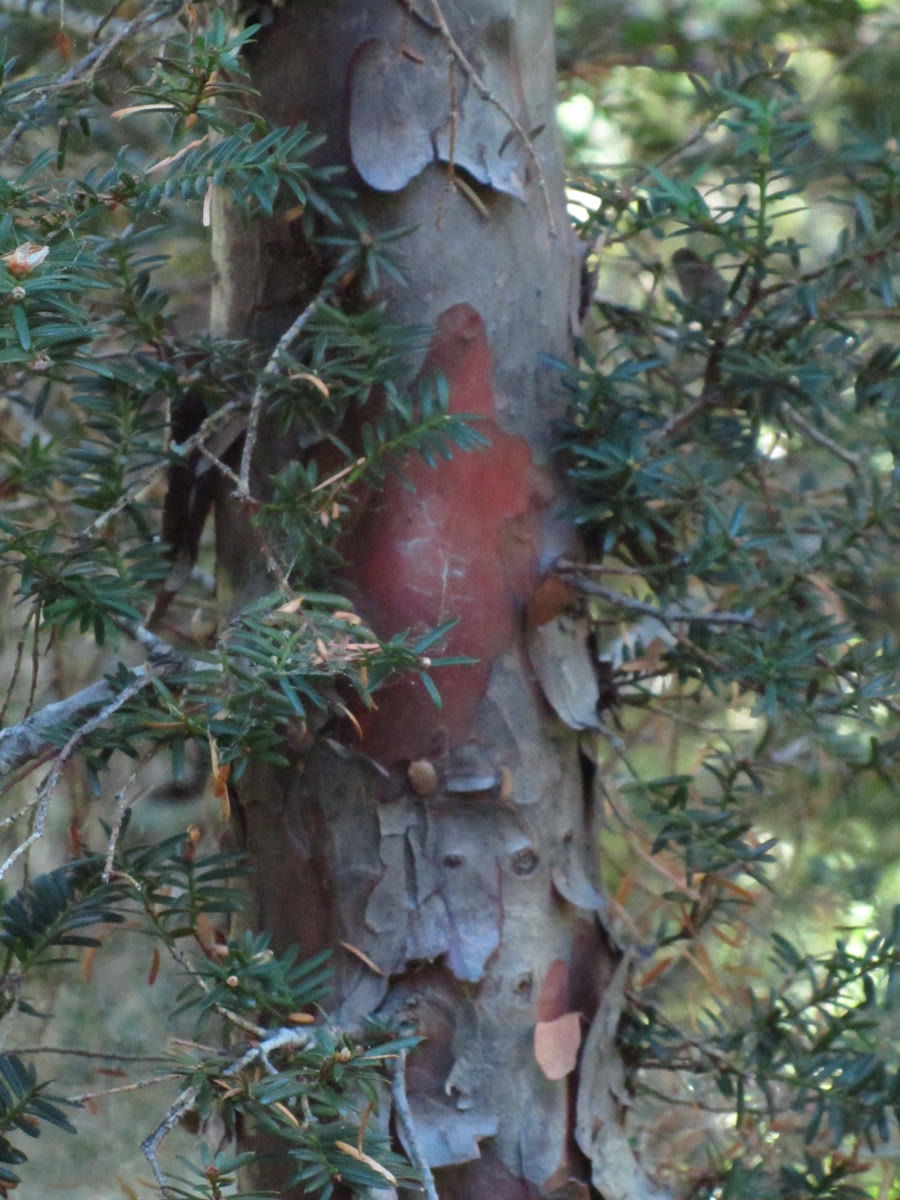
\includegraphics[width=0.32\linewidth]{images/book4/pacific-yew.jpg}

{\small पैसिफ़िक यू की छाल और पत्तियाँ, पैक्लिटैक्सेल का पहला स्रोत।
छायाचित्र: जो ब्लोवे, CC BY-SA 2.0।}
\end{omfigure}

\section{किसी संश्लेषण को मापना}

\begin{definition}[पूर्ण संश्लेषण]\label{def:b3:total-synthesis:total}
\emph{पूर्ण संश्लेषण}\index{पूर्ण संश्लेषण} किसी जटिल अणु को, प्रायः किसी
प्राकृतिक उत्पाद को, सरल व्यावसायिक यौगिकों से बनाता है। \emph{औपचारिक
संश्लेषण}\index{औपचारिक संश्लेषण} किसी पूर्ववर्ती पूर्ण संश्लेषण का कोई मध्यवर्ती
बनाता है, जिससे मार्ग काग़ज़ पर पूरा हो जाता है। \emph{अर्धसंश्लेषण}\index{अर्धसंश्लेषण}
किसी ऐसे प्राकृतिक यौगिक से आरंभ होता है जो पहले से लक्ष्य के निकट हो।
\end{definition}

\begin{definition}[मार्ग की संरचना]\label{def:b3:total-synthesis:architecture}
\emph{रैखिक संश्लेषण}\index{रैखिक संश्लेषण} में प्रत्येक चरण पिछले चरण के
उत्पाद पर कार्य करता है; \emph{अभिसारी संश्लेषण}\index{अभिसारी संश्लेषण} में
अलग-अलग खंड समानांतर रूप से बनाए जाते हैं और देर से जोड़े जाते हैं।
\emph{सबसे लंबा रैखिक अनुक्रम}\index{सबसे लंबा रैखिक अनुक्रम} (LLS) किसी भी आरंभिक
पदार्थ से लक्ष्य तक चरणों की सबसे बड़ी संख्या है। \emph{समग्र
लब्धि}\index{समग्र लब्धि} प्राप्त लक्ष्य की मात्रा को सीमांत आरंभिक पदार्थ की
मात्रा से भाग देने पर मिलती है।
\end{definition}

\begin{proposition}[समग्र लब्धि]\label{prop:b3:total-synthesis:overall-yield}
$y_1, \dots, y_n$ लब्धियों वाले चरणों के अनुक्रम के लिए \omterm{def:b3:total-synthesis:architecture}{समग्र लब्धि} $Y = \prod_i y_i$ है।
\end{proposition}

\begin{proof}
प्रत्येक चरण उसे मिली मात्रा को उसके $y_i$ गुना उत्पाद में बदलता है; लक्ष्य तक
पहुँचने वाली मात्रा आरंभिक मात्रा को बारी-बारी से प्रत्येक गुणक से गुणा करने पर
मिलती है।
\end{proof}

\begin{proposition}[अभिसरण]\label{prop:b3:total-synthesis:convergent}
$n = 2m + 1$ चरणों का मार्ग, प्रत्येक की समान लब्धि $y$, जो $m$ चरणों की दो शाखाओं के रूप में बना हो
और एक युग्मन चरण से जुड़ा हो, अपने सबसे लंबे रैखिक अनुक्रम के अनुदिश \omterm{def:b3:total-synthesis:architecture}{समग्र लब्धि} $y^{m+1}$ रखता है,
जबकि उन्हीं चरणों के रैखिक मार्ग के लिए यह $y^{2m+1}$ है।
\end{proposition}

\begin{proof}
प्रत्येक शाखा अलग से, जितना आवश्यक हो उतने आरंभिक पदार्थ पर, बनाई जाती है:
प्रत्येक शाखा का पदार्थ $m$ चरणों से और फिर युग्मन से गुज़रता है, $m + 1$
गुणक $y$। रैखिक मार्ग में पदार्थ सभी $2m + 1$ से गुज़रता है। $m = 10$
और $y = 0.90$ के लिए: 31\,\% बनाम 11\,\%।
\end{proof}

\begin{omfigure}
\begin{tikzpicture}
\begin{axis}[width=0.7\linewidth, height=5.8cm, xmin=0, xmax=30, ymin=0, ymax=1.02,
  axis lines=left, xlabel={चरणों की संख्या $n$}, ylabel={समग्र लब्धि},
  tick label style={font=\scriptsize}, label style={font=\small},
  legend style={font=\scriptsize, draw=none, at={(1.03,0.5)}, anchor=west}, legend cell align=left]
\addplot[color=omDef, thick] table[x=n, y=y95] {figdata/out/bachelor-3-overall-yield.dat};
\addlegendentry{95\,\% प्रति चरण}
\addplot[color=omMeth, thick] table[x=n, y=y90] {figdata/out/bachelor-3-overall-yield.dat};
\addlegendentry{90\,\%}
\addplot[color=omThm, thick] table[x=n, y=y80] {figdata/out/bachelor-3-overall-yield.dat};
\addlegendentry{80\,\%}
\addplot[color=omMeth, thick, dashed, mark=*, mark size=1pt] table[x=n, y=y90] {figdata/out/bachelor-3-overall-yield-b.dat};
\addlegendentry{90\,\%, अभिसारी}
\end{axis}
\end{tikzpicture}

{\small तीन प्रति-चरण लब्धियों के लिए चरणों की संख्या के विरुद्ध \omterm{def:b3:total-synthesis:architecture}{समग्र लब्धि}
(ठोस: रैखिक मार्ग), और 90\,\% प्रति चरण पर अभिसारी मार्गों के लिए (अंतिम चरण में
जुड़ी दो समान शाखाएँ; खंडित)। 90\,\% पर बीस चरण 12\,\% छोड़ते हैं; वही
चरण अभिसारी रूप से व्यवस्थित करने पर लगभग तीन गुना अधिक छोड़ते हैं।}
\end{omfigure}

\begin{omfigure}
\begin{tikzpicture}[font=\scriptsize, >=Stealth, node distance=0.9cm,
  st/.style={circle, draw, fill=omDef!15, minimum size=4mm, inner sep=0pt}]
  \foreach \i in {0,...,6} { \node[st] (l\i) at (\i*0.9,1.6) {}; }
  \foreach \i in {0,...,5} { \pgfmathtruncatemacro\j{\i+1} \draw[->] (l\i) -- (l\j); }
  \node[anchor=west] at (6.0,1.6) {रैखिक: 6 चरण, LLS 6};
  \foreach \i in {0,...,2} { \node[st] (a\i) at (\i*0.9,0.6) {}; \node[st] (b\i) at (\i*0.9,-0.6) {}; }
  \draw[->] (a0) -- (a1); \draw[->] (a1) -- (a2); \draw[->] (b0) -- (b1); \draw[->] (b1) -- (b2);
  \node[st, fill=omThm!25] (t) at (3.0,0) {};
  \draw[->] (a2) -- (t); \draw[->] (b2) -- (t);
  \node[anchor=west] at (3.4,0) {अभिसारी: 5 चरण, LLS 3};
\end{tikzpicture}

{\small मार्ग-वृक्ष: प्रत्येक वृत्त एक यौगिक है, प्रत्येक तीर एक चरण। रैखिक मार्ग
अपना सारा पदार्थ प्रत्येक चरण से गुज़ारता है; अभिसारी मार्ग दो खंड
साथ-साथ बनाकर उन्हें युग्मित करता है, जिससे उसका \omterm{def:b3:total-synthesis:architecture}{सबसे लंबा रैखिक अनुक्रम} छोटा होता है।}
\end{omfigure}

\begin{definition}[मितव्ययिताएँ और आदर्शता]\label{def:b3:total-synthesis:economy}
\emph{चरण मितव्ययिता}\index{चरण मितव्ययिता} लक्ष्य तक यथासंभव कम चरणों में
पहुँचने का उद्देश्य है; \emph{रक्षी-समूह मितव्ययिता}\index{रक्षी-समूह मितव्ययिता},
यथासंभव कम रक्षण और विरक्षण चरणों का उपयोग करने का। किसी मार्ग की
\emph{आदर्शता}\index{आदर्शता} उसके उन चरणों का अंश है जो
ढाँचा बनाते हैं या ऑक्सीकरण स्तर में कोई आवश्यक परिवर्तन करते हैं:
$(\text{निर्माण चरण} + \text{रणनीतिक अपचयोपचय चरण})/(\text{कुल चरण})$।
\end{definition}

\begin{proposition}[किसी मार्ग की आदर्शता]\label{prop:b3:total-synthesis:ideality}
एक-पात्र मार्ग जो केवल ढाँचे के आबंध बनाता है, उसकी \omterm{def:b3:total-synthesis:economy}{आदर्शता} 100\,\% है; प्रत्येक रक्षण,
विरक्षण, क्रियात्मक-समूह अंतर्रूपांतरण या गैर-रणनीतिक अपचयोपचय चरण
उसे घटाता है।
\end{proposition}

\begin{proof}
सीधे परिभाषा से: ऐसे चरण अंश में जोड़े बिना हर में
जुड़ते हैं।
\end{proof}

\section{रक्षी समूह और उनकी मितव्ययिता}

प्रत्येक रक्षी समूह की कीमत कम से कम दो चरण होती है, उसे लगाने और
हटाने के अभिकर्मक, और दोनों में खोया पदार्थ। 90\,\% पर आठ चरणों का मार्ग
अपने पदार्थ का 43\,\% बचाता है; 95\,\% प्रत्येक पर दो रक्षण और दो विरक्षण जोड़ने से
यह 35\,\% रह जाता है। रक्षी समूह लांबिक चुने जाते हैं, ताकि प्रत्येक को
अन्य को छुए बिना हटाया जा सके; इससे भी अच्छा, चरणों का क्रम ऐसा
व्यवस्थित किया जाता है कि जब क्रियाशील समूह बाधा डालता, तब वह उपस्थित ही न हो, या अभी
प्रकट न हुआ हो: रक्षी-समूह-मुक्त संश्लेषण एक लक्ष्य हैं, कौतूहल नहीं।

\begin{method}[किसी पूर्ण संश्लेषण को पढ़ना]\label{met:b3:total-synthesis:analyse}
\begin{enumerate}
  \item लक्ष्य के वलय, त्रिविमजनक केंद्र और संवेदनशील समूह पहचानिए।
  \item मुख्य विच्छेदन और अग्र दिशा में उन्हें बनाने वाली अभिक्रियाएँ खोजिए
        (\omterm{def:b3:total-synthesis:strategic-bond}{रणनीतिक आबंध})।
  \item चरण गिनिए और \omterm{def:b3:total-synthesis:architecture}{सबसे लंबा रैखिक अनुक्रम} खोजिए; अभिसरण पर ध्यान दीजिए।
  \item ध्यान दीजिए कि प्रत्येक त्रिविमजनक केंद्र कैसे स्थापित होता है (क्रियाधार नियंत्रण, सहायक, उत्प्रेरक,
        \omterm{def:b3:asymmetric-synthesis:chiral-pool}{किरैल कुंड})।
  \item रक्षी समूहों और अन्य अनादर्श चरणों की सूची बनाइए; \omterm{def:b3:total-synthesis:architecture}{समग्र
        लब्धि} और \omterm{def:b3:total-synthesis:economy}{आदर्शता} परिकलित कीजिए।
\end{enumerate}
\end{method}

\begin{method}[चरण गिनना]\label{met:b3:total-synthesis:count}
\begin{enumerate}
  \item एक चरण वह एक संक्रिया है जो किसी पृथक किए गए (या कम से कम उपचार-पश्चात् प्रक्रिया से गुज़रे)
        उत्पाद पर समाप्त होती है; पृथक्करण के बिना एक-पात्र अनुक्रम एक चरण गिना जाता है।
  \item कुल के लिए सभी चरण गिनिए; LLS के लिए, किसी
        व्यावसायिक यौगिक से लक्ष्य तक का सबसे लंबा पथ अपनाइए।
  \item \omterm{def:b3:total-synthesis:architecture}{समग्र लब्धि} के लिए LLS के अनुदिश लब्धियों को गुणा कीजिए।
\end{enumerate}
\end{method}

\section{रणनीतिक आबंध और वलय बनाने वाले मुख्य चरण}

\begin{definition}[रणनीतिक आबंध]\label{def:b3:total-synthesis:strategic-bond}
किसी लक्ष्य का \emph{रणनीतिक आबंध} वह आबंध है\index{रणनीतिक आबंध} जिसका
विच्छेदन लक्ष्य को सबसे अधिक सरल बनाता है, प्रायः किसी वलय-तंत्र को विभाजित करके
या कई त्रिविमजनक केंद्रों को एक साथ हटाकर, और जिसे कोई विश्वसनीय अभिक्रिया
बना सकती है।
\end{definition}

एक साथ दो आबंध या कई त्रिविमजनक केंद्र बनाने वाली वलय-निर्माण अभिक्रियाएँ
मुख्य आधार हैं: डील्स--ऐल्डर अभिक्रिया (दो C--C आबंध, चार तक
त्रिविमजनक केंद्र, त्रिविमविशिष्ट रूप से, \cref{ch:b3:pericyclic}), रॉबिन्सन
वलयन (किसी कीटोन पर एक छह-सदस्यीय वलय), मध्यम और बड़े वलयों के लिए \omterm{def:b3:homogeneous-catalysis:metathesis}{वलय-समापी मेटाथीसिस}
(\cref{ch:b3:homogeneous-catalysis}), और \omterm{def:b3:total-synthesis:cascade}{सोपानी अभिक्रियाएँ}।

\begin{definition}[सोपानी अभिक्रिया]\label{def:b3:total-synthesis:cascade}
\emph{सोपानी अभिक्रिया}\index{सोपानी अभिक्रिया} रूपांतरणों का ऐसा
अनुक्रम है जिसमें प्रत्येक चरण अगले के लिए क्रियात्मकता उत्पन्न करता है,
मध्यवर्तियों को पृथक किए बिना या अभिकर्मक मिलाए बिना।
\end{definition}

\begin{definition}[जैवअनुकारी संश्लेषण]\label{def:b3:total-synthesis:biomimetic}
\emph{जैवअनुकारी संश्लेषण}\index{जैवअनुकारी संश्लेषण} उस मार्ग का अनुकरण करता है
जिससे किसी प्राकृतिक उत्पाद को जीव में बनाया जाना माना जाता है।
\end{definition}

कोशिकाओं में स्क्वैलीन ऑक्साइड का लैनोस्टेरॉल में चक्रीकरण, एक एंज़ाइमी सोपान में चार वलय और सात
त्रिविमजनक केंद्र, ने विलियम जॉनसन के पॉलिईन चक्रीकरणों को प्रेरित किया, जिनमें
सावधानी से अभिकल्पित पॉलिईन के एक सिरे पर आरंभ हुआ एक धनायन कुर्सी-सदृश संक्रमण
अवस्थाओं से होकर वलय पर वलय बंद करता जाता है, और स्टेरॉयडों के
\textit{trans} वलय-संगलन स्थापित करता है।

\section{युगांतरकारी मार्ग}

\begin{definition}[मैनिख अभिक्रिया]\label{def:b3:total-synthesis:mannich}
\emph{मैनिख अभिक्रिया}\index{मैनिख अभिक्रिया} किसी ईनॉल या ईनोलेट का एक
इमीनियम आयन पर योग है, जो किसी ऐल्डिहाइड और एक प्राथमिक या द्वितीयक
ऐमीन से अभिक्रिया-मिश्रण में ही बनता है, जिससे एक $\beta$-ऐमीनो कार्बोनिल यौगिक मिलता है।
\end{definition}

1917 में रॉबर्ट रॉबिन्सन ने ऐट्रोपीन और कोकेन का द्विचक्रीय क्रोड, ट्रोपिनोन,
तीन सरल घटकों से जल में एक ही पात्र में बनाया, यह कल्पना करते हुए कि
पौधा भी इसे इसी तरह बनाता होगा:
$\ce{C4H6O2 + CH3NH2 + C5H6O5 -> C8H13NO + 2CO2 + 2H2O}$ (सक्सिनैल्डिहाइड, मेथिलऐमीन और
ऐसीटोनडाइकार्बोक्सिलिक अम्ल ट्रोपिनोन देते हैं)।

\begin{omfigure}
\begin{tikzpicture}[font=\small, >=Stealth]
  \node[align=center] at (-0.5,0) {$\ce{OHC-CH2CH2-CHO}$\\ $+\ \ce{CH3NH2}$\\ $+\ \ce{HO2C-CH2-CO-CH2-CO2H}$};
  \draw[->, thick] (3.0,0) -- (4.7,0) node[midway, above, font=\scriptsize] {बफ़रित जल} node[midway, below, font=\scriptsize] {$-\ce{2CO2}$, $-\ce{2H2O}$};
  \begin{scope}[xshift=6.1cm, yshift=-0.2cm]
    \coordinate (c1) at (-1,0.3); \coordinate (c2) at (-0.8,-0.5); \coordinate (c3) at (0,-0.9);
    \coordinate (c4) at (0.8,-0.5); \coordinate (c5) at (1,0.3); \coordinate (c6) at (0.45,1.15);
    \coordinate (c7) at (-0.45,1.15); \coordinate (n) at (0,0.45);
    \draw[thick] (c1) -- (c2) -- (c3) -- (c4) -- (c5) -- (c6);
    \draw[thick] (c7) -- (c1);
    \draw[thick] (c6) -- (0.12,1.15); \draw[thick] (-0.12,1.15) -- (c7);
    \draw[thick] (c1) -- (n) -- (c5);
    \draw[thick] (n) -- (0,1.6) node[above, inner sep=1pt] {$\ce{CH3}$};
    \draw[thick, double, double distance=1.5pt] (c3) -- (0,-1.55) node[below, inner sep=1pt] {O};
    \node[fill=white, inner sep=0.5pt] at (n) {N};
    \node[font=\scriptsize, anchor=west] at (1.2,0.3) {ट्रोपिनोन};
  \end{scope}
\end{tikzpicture}

{\small रॉबिन्सन का ट्रोपिनोन संश्लेषण। दो \omterm{def:b3:total-synthesis:mannich}{मैनिख अभिक्रियाएँ}, पहली
अंतराआण्विक और दूसरी वलय बंद करने वाली, तीनों घटकों को जोड़ती हैं;
वे दो कार्बोक्सिलिक अम्ल समूह जिन्होंने केंद्रीय $\ce{CH2}$ समूहों को ईनॉलन-योग्य बनाया था, फिर
कार्बन डाइऑक्साइड के रूप में निकल जाते हैं। द्विचक्रीय उत्पाद में N-मेथिल सेतु
सप्तसदस्यीय वलय के आर-पार फैला है।}
\end{omfigure}

\begin{proposition}[एक पात्र में ट्रोपिनोन]\label{prop:b3:total-synthesis:tropinone}
एक-पात्र ट्रोपिनोन संश्लेषण दो \omterm{def:b3:total-synthesis:mannich}{मैनिख अभिक्रियाएँ} हैं जिनके बाद दो
विकार्बोक्सिलन होते हैं।
\end{proposition}

\begin{proof}[तर्क]
मेथिलऐमीन और सक्सिनैल्डिहाइड का एक ऐल्डिहाइड समूह एक इमीनियम आयन देते हैं;
ऐसीटोनडाइकार्बोक्सिलिक अम्ल का एक ईनॉल उस पर जुड़ता है (पहली मैनिख)। बना हुआ द्वितीयक
ऐमीन दूसरे ऐल्डिहाइड समूह के साथ संघनित होकर एक चक्रीय इमीनियम
आयन बनाता है, जिस पर कीटोन के दूसरी ओर का ईनॉल आक्रमण करता है (दूसरी मैनिख),
जिससे द्विचक्र बंद हो जाता है। फिर दोनों $\beta$-कीटो अम्ल समूह $\ce{CO2}$ खो देते हैं, जैसा $\beta$-कीटो अम्ल
हल्का गर्म करने पर करते हैं।
\end{proof}

इलायस कोरी के प्रोस्टाग्लैंडिन $\mathrm F_{2\alpha}$ संश्लेषण (1969) ने पश्च-संश्लेषी विश्लेषण को
सुस्पष्ट बनाया। डील्स--ऐल्डर अभिक्रिया से बना एक बाइसाइक्लो[2.2.1]हेप्टीनोन
साइक्लोपेन्टेन के प्रतिस्थापियों का आपेक्षिक विन्यास वहन करता है; एक
\omterm{def:b3:radicals-carbenes:baeyer}{बायर--विलिगर ऑक्सीकरण} (\cref{ch:b3:radicals-carbenes}) और एक
आयोडोलैक्टोनन इसे कोरी लैक्टोन में बदल देते हैं, जिससे दोनों पार्श्व शृंखलाएँ
ओलेफ़िनन द्वारा जोड़ी जाती हैं। यह लैक्टोन तब से अनेक प्रोस्टाग्लैंडिन
औषधों के लिए काम आया है।

\begin{omfigure}
\begin{tikzpicture}[font=\small,
  box/.style={draw, rounded corners, align=center, fill=omDef!8, inner sep=4pt}]
  \node[box] (t) at (0,0) {प्रोस्टाग्लैंडिन\\ $\mathrm F_{2\alpha}$};
  \node[box] (l) at (4.4,0) {कोरी लैक्टोन\\ (चार\\ त्रिविमजनक केंद्र)};
  \node[box] (b) at (9.2,0) {बाइसाइक्लो[2.2.1]-\\ हेप्टीनोन};
  \node[box] (d) at (9.2,-2.4) {प्रतिस्थापित\\ साइक्लोपेन्टाडाईन $+$\\ कीटीन तुल्य};
  \draw[omretro] (t) -- (l) node[midway, above=3pt, font=\scriptsize] {ओलेफ़िनन};
  \draw[omretro] (l) -- (b) node[midway, above=3pt, font=\scriptsize, align=center] {आयोडोलैक्टोनन,\\ बायर--विलिगर};
  \draw[omretro] (b) -- (d) node[midway, right, font=\scriptsize] {डील्स--ऐल्डर};
\end{tikzpicture}

{\small कोरी का प्रोस्टाग्लैंडिन $\mathrm F_{2\alpha}$ का पश्च-संश्लेषण, रूपरेखा में (द्वि-तीर: ``से
बनता है'')। दोनों पार्श्व शृंखलाएँ पहले विच्छेदित की जाती हैं; अपने चार त्रिविमजनक
केंद्रों सहित साइक्लोपेन्टेन एक लैक्टोन से आता है, लैक्टोन एक द्विचक्रीय कीटोन से,
और कीटोन एक डील्स--ऐल्डर अभिक्रिया से जो उनका आपेक्षिक
विन्यास निर्धारित करती है।}
\end{omfigure}

इन्फ़्लुएंज़ा की औषध ओसेल्टामिविर औद्योगिक रूप से शिकिमिक अम्ल से बनाई जाती है, जो
चक्रफूल (स्टार ऐनीस) से निष्कर्षित और बाद में किण्वन द्वारा उत्पादित एक किरैल-कुंड यौगिक है:
इसका छह-सदस्यीय वलय और त्रिविमजनक केंद्र पहले से अपने स्थान पर हैं।
मार्ग वलय-डाइऑल को एक एपॉक्साइड में बदलता है, उसे ऐज़ाइड से खोलता है, एक
ऐज़िरिडीन बंद करता है और उसे फिर ऐज़ाइड से खोलता है, जिससे दोनों नाइट्रोजन परमाणु
\textit{trans} स्थापित होते हैं; ऐसीटिलन और अपचयन काम पूरा करते हैं। चूँकि सोडियम ऐज़ाइड और
कार्बनिक ऐज़ाइड विषैले हैं और बड़े पैमाने पर संभावित रूप से विस्फोटक, बाद में ऐज़ाइड-मुक्त
मार्ग विकसित किए गए।

\begin{omfigure}
\begin{tikzpicture}[font=\scriptsize, >=Stealth,
  box/.style={draw, rounded corners, align=center, fill=omMeth!8, inner sep=3pt}]
  \node[box] (a) at (0,0) {($-$)-शिकिमिक अम्ल\\ (किरैल कुंड)};
  \node[box] (b) at (3.1,0) {एस्टर, कीटल,\\ मेसिलेट};
  \node[box] (c) at (6.0,0) {एपॉक्साइड};
  \node[box] (d) at (8.6,0) {ऐज़िडो ऐल्कोहॉल};
  \node[box] (e) at (8.6,-1.5) {ऐज़िरिडीन};
  \node[box] (f) at (5.4,-1.5) {\textit{trans}-डाइऐमीन\\ पूर्वगामी (ऐज़ाइड)};
  \node[box] (g) at (1.6,-1.5) {ओसेल्टामिविर\\ फ़ॉस्फ़ेट};
  \draw[->] (a) -- (b); \draw[->] (b) -- (c); \draw[->] (c) -- (d) node[midway, above] {$\ce{N3-}$};
  \draw[->] (d) -- (e); \draw[->] (e) -- (f) node[midway, above] {$\ce{N3-}$};
  \draw[->] (f) -- (g) node[midway, below, align=center] {ऐसीटिलन,\\ अपचयन};
\end{tikzpicture}

{\small शिकिमिक अम्ल से ओसेल्टामिविर, केवल मुख्य चरण: प्राकृतिक वलय और उसके
त्रिविमजनक केंद्र बनाए रखे जाते हैं, और एक एपॉक्साइड और एक ऐज़िरिडीन को ऐज़ाइड से
क्रमशः खोलकर दो नाइट्रोजन परमाणु एक-दूसरे के \textit{trans} प्रविष्ट किए जाते हैं।}
\end{omfigure}

\section{खोज से प्रक्रम तक}

जैविक परीक्षण के लिए मिलीग्राम देने वाला मार्ग शायद ही कभी वही होता है जो
टनों के लिए प्रयुक्त हो। प्रक्रम रसायनज्ञ लागत, सुरक्षा और दृढ़ता के लिए मार्गों की छानबीन करते हैं:
वे क्रिस्टलन के पक्ष में वर्णलेखन हटाते हैं, संकटपूर्ण
अभिकर्मकों और निम्नतापी तापों को बदलते हैं, अनुक्रम छोटा करते हैं, प्रत्येक चरण की तापीय
सुरक्षा ऊष्मामिति से जाँचते हैं, और अशुद्धियों के लिए विनिर्देश तय करते हैं।
ये विकल्प \cref{ch:b3:green-industrial} के मापों से मिलते हैं।

\begin{inthelab}[एक ग्राम से एक किलोग्राम तक]
गोल पेंदी वाले फ़्लास्क में एक ग्राम पर चलाया गया चरण दस ग्राम पर एक
जैकेट-युक्त रिएक्टर में दोहराया जाता है, जिसमें ऊपर से लगा विलोडक और द्रव में एक
ताप-प्रोब होता है, और आंतरिक ताप पर नज़र रखते हुए क्रियाशील अभिकर्मक नियंत्रित दर से
मिलाया जाता है: मुक्त ऊष्मा आयतन के साथ बढ़ती है, परंतु उसे हटाने वाला
क्षेत्रफल आकार के केवल वर्ग के साथ बढ़ता है। जब ऊष्मा प्रवाह और उपचार-पश्चात् प्रक्रिया
(प्रावस्था पृथक्करण, निस्यंदन, शुष्कन) ठीक व्यवहार करते हैं, तभी चरण को किलोग्राम पर चलाया जाता है।
\end{inthelab}

\begin{safety}{\ghs[0.62cm]{GHS06}\ghs[0.62cm]{GHS08}\ghs[0.62cm]{GHS09}}
% ledger: ghs4:NaN3
सोडियम ऐज़ाइड: निगलने पर घातक, जलीय जीवों के लिए अत्यधिक विषैला; अम्लों के साथ यह
हाइड्रैज़ोइक अम्ल मुक्त करता है, एक विषैली और विस्फोटक गैस, और भारी धातुओं
(नालियों में कॉपर और लेड) के साथ विस्फोटक ऐज़ाइड बनाता है। अपशिष्ट को
रासायनिक रूप से नष्ट किया जाता है, कभी बहाया नहीं जाता।
\end{safety}

\begin{history}[रॉबिन्सन, वुडवर्ड, कोरी]
रॉबर्ट रॉबिन्सन को ऐल्कलॉइडों और अन्य पादप उत्पादों पर उनके कार्य के लिए 1947 का
रसायन का नोबेल पुरस्कार मिला; 1917 का उनका ट्रोपिनोन संश्लेषण अपनी मितव्ययिता के लिए
आज भी उद्धृत किया जाता है। रॉबर्ट वुडवर्ड के क्विनीन, कोलेस्टेरॉल,
क्लोरोफ़िल और, ऐल्बर्ट एशेनमोज़र के साथ, विटामिन $\mathrm B_{12}$ के संश्लेषणों ने \omterm{def:b3:total-synthesis:total}{पूर्ण संश्लेषण} को एक कला बना दिया
(1965 का पुरस्कार)। इलायस कोरी ने पश्च-संश्लेषी विश्लेषण को औपचारिक रूप दिया और
कार्बनिक संश्लेषण के सिद्धांत और कार्यप्रणाली के लिए 1990 का पुरस्कार पाया।
\end{history}

\section{अभ्यास}

\begin{exercise}[$\star$]\label{exo:b3:total-synthesis:1}
90\,\% और 80\,\% प्रति चरण पर 10- और 20-चरणीय रैखिक मार्गों की \omterm{def:b3:total-synthesis:architecture}{समग्र लब्धि}
परिकलित कीजिए।
\end{exercise}

\begin{exercise}[$\star$]\label{exo:b3:total-synthesis:2}
एक मार्ग खंड A को पाँच चरणों में और खंड B को तीन में बनाता है, उन्हें युग्मित करता है, और
लक्ष्य तक चार और चरण लेता है। चरणों की कुल संख्या और
\omterm{def:b3:total-synthesis:architecture}{सबसे लंबा रैखिक अनुक्रम} बताइए।
\end{exercise}

\begin{exercise}[$\star$]\label{exo:b3:total-synthesis:3}
ऐसीटोन, मेथेनैल (फ़ॉर्मैल्डिहाइड) और डाइमेथिलऐमीन की \omterm{def:b3:total-synthesis:mannich}{मैनिख अभिक्रिया} का उत्पाद
बताइए।
\end{exercise}

\begin{exercise}[$\star$]\label{exo:b3:total-synthesis:4}
4-ऐसीटिलसाइक्लोहेक्सीन का एक डील्स--ऐल्डर विच्छेदन बताइए, और अग्र
अभिक्रिया।
\end{exercise}

\begin{exercise}[$\star\star$]\label{exo:b3:total-synthesis:5}
एक 21-चरणीय रैखिक मार्ग 90\,\% प्रति चरण पर चलता है। उसकी \omterm{def:b3:total-synthesis:architecture}{समग्र लब्धि} परिकलित कीजिए, और
दो 10-चरणीय शाखाओं और एक युग्मन वाले अभिसारी संस्करण की भी।
\end{exercise}

\begin{exercise}[$\star\star$]\label{exo:b3:total-synthesis:6}
मार्ग A में 12 चरण हैं, जिनमें से 7 ढाँचे के आबंध बनाते हैं और 1 एक रणनीतिक
अपचयन है; मार्ग B में 9 चरण हैं, जिनमें से 7 ढाँचे के। उनकी \omterm{def:b3:total-synthesis:economy}{आदर्शताएँ} परिकलित कीजिए।
\end{exercise}

\begin{exercise}[$\star\star$]\label{exo:b3:total-synthesis:7}
90\,\% प्रति चरण वाले आठ-चरणीय मार्ग को दो रक्षी समूह चाहिए, प्रत्येक 95\,\% पर लगाया और
हटाया जाता है। उनके साथ और उनके बिना \omterm{def:b3:total-synthesis:architecture}{समग्र लब्धि} परिकलित कीजिए।
\end{exercise}

\begin{exercise}[$\star\star$]\label{exo:b3:total-synthesis:8}
एक ट्राइऑल में एक प्राथमिक, एक द्वितीयक और एक तृतीयक हाइड्रॉक्सी समूह है। ऐसे
रक्षी समूह प्रस्तावित कीजिए जिनसे प्रत्येक को बारी-बारी से मुक्त किया जा सके, और उन्हें हटाने की
परिस्थितियाँ बताइए।
\end{exercise}

\begin{exercise}[$\star\star$]\label{exo:b3:total-synthesis:9}
पैक्लिटैक्सेल का उत्पादन उसके किसी भी \omterm{def:b3:total-synthesis:total}{पूर्ण
संश्लेषण} के बजाय \omterm{def:b3:total-synthesis:total}{अर्धसंश्लेषण} से क्यों किया गया?
\end{exercise}

\begin{exercise}[$\star\star\star$]\label{exo:b3:total-synthesis:10}
2-मेथिलसाइक्लोहेक्सेन-1,3-डाइओन मेथिल वाइनिल कीटोन से रॉबिन्सन
वलयन में अभिक्रिया करता है। माइकल और ऐल्डोल चरण पहचानिए और बनने वाला द्विचक्रीय ईनोन
(वीलैंड--मीशर कीटोन) बताइए।
\end{exercise}

\begin{exercise}[$\star\star\star$]\label{exo:b3:total-synthesis:11}
दिखाइए कि \cref{prop:b3:total-synthesis:convergent} का अभिसारी मार्ग रैखिक मार्ग से
$y^{-m}$ गुना अधिक पदार्थ बचाता है, और 90\,\% पर $m = 5$ तथा
$m = 15$ के लिए इस गुणक का मान निकालिए।
\end{exercise}

\begin{exercise}[$\star\star\star$]\label{exo:b3:total-synthesis:12}
किसी पॉलिईन चक्रीकरण में कुर्सी-सदृश संक्रमण अवस्थाएँ \textit{trans} वलय-संगलन
क्यों देती हैं, और प्रत्येक द्विबंध की ज्यामिति (\textit{E} या \textit{Z}) क्यों महत्त्वपूर्ण है?
\end{exercise}

\section{समस्या: एक पात्र में ट्रोपिनोन}

\begin{problem}[{सप्ताहांत समस्या --- एक पात्र में ट्रोपिनोन: तीन घटक
और संतुलित समीकरण, दो मैनिख अभिक्रियाएँ, एक लंबे
रैखिक मार्ग से तुलना, और ट्रोपिनोन तथा उसके अपचयन उत्पादों का त्रिविम रसायन}]
\label{pb:b3:total-synthesis:1}
% ledger: aw:C, aw:H, aw:N, aw:O
समस्या के आँकड़े: pH 5 के निकट बफ़रित जल में चलाया गया एक-पात्र संश्लेषण
42\,\% लब्धि में ट्रोपिनोन देता है; एक पुराने रैखिक मार्ग को औसतन 75\,\% वाले 14 चरण चाहिए।

\medskip\noindent\textbf{भाग I --- घटक और समीकरण।}
\begin{enumerate}
  \item सक्सिनैल्डिहाइड, मेथिलऐमीन, ऐसीटोनडाइकार्बोक्सिलिक अम्ल
        और ट्रोपिनोन के सूत्र बताइए।
  \item संतुलित समीकरण लिखिए।
  \item अभिकारकों और ट्रोपिनोन के मोलर द्रव्यमान परिकलित कीजिए।
  \item परमाणु मितव्ययिता परिकलित कीजिए।
  \item ऐसीटोन के स्थान पर ऐसीटोनडाइकार्बोक्सिलिक अम्ल क्यों प्रयुक्त होता है?
  \item उदासीन pH के निकट बफ़र करना क्यों सहायक है?
\end{enumerate}

\medskip\noindent\textbf{भाग II --- क्रियाविधि।}
\begin{enumerate}[resume]
  \item पहले इमीनियम आयन का बनना लिखिए।
  \item पहली \omterm{def:b3:total-synthesis:mannich}{मैनिख अभिक्रिया} दर्शाइए।
  \item दूसरा इमीनियम आयन कैसे बनता है?
  \item दूसरी, वलय-समापी \omterm{def:b3:total-synthesis:mannich}{मैनिख अभिक्रिया} दर्शाइए।
  \item दोनों कार्बोक्सिलिक अम्ल समूह $\ce{CO2}$ के रूप में क्यों निकलते हैं?
  \item बनने वाले C--C और C--N आबंध गिनिए।
\end{enumerate}

\medskip\noindent\textbf{भाग III --- एक पात्र बनाम चौदह चरण।}
\begin{enumerate}[resume]
  \item रैखिक मार्ग की \omterm{def:b3:total-synthesis:architecture}{समग्र लब्धि} परिकलित कीजिए।
  \item उसकी तुलना में एक-पात्र लब्धि का अनुपात परिकलित कीजिए।
  \item एक-पात्र मार्ग की \omterm{def:b3:total-synthesis:economy}{आदर्शता} परिकलित कीजिए।
  \item लब्धि के अतिरिक्त और क्या एक-पात्र मार्ग के पक्ष में है?
  \item एक-पात्र संश्लेषण को जैवअनुकारी क्यों कहा जाता है?
  \item इस अध्याय का कोई अन्य अभिक्रिया-वर्ग बताइए जो एक साथ कई आबंध बनाता है।
\end{enumerate}

\medskip\noindent\textbf{भाग IV --- त्रिविम रसायन।}
\begin{enumerate}[resume]
  \item क्या ट्रोपिनोन किरैल है? उसका \omterm{def:b3:point-groups:operation}{सममिति तत्व} खोजिए।
  \item फिर भी दोनों सेतुशीर्ष कार्बन त्रिविमजनक केंद्र क्यों हैं?
  \item कीटोन का अपचयन दो ऐल्कोहॉल देता है, ट्रोपीन और स्यूडोट्रोपीन। उनका
        संबंध क्या है?
  \item क्या ट्रोपीन और स्यूडोट्रोपीन किरैल हैं?
  \item कोई हाइड्राइड कार्बोनिल समूह के पास वरीयता से एक फलक से क्यों पहुँचता है?
  \item परिणाम बताइए: एक-पात्र लब्धि का रैखिक मार्ग की
        \omterm{def:b3:total-synthesis:architecture}{समग्र लब्धि} से अनुपात।
\end{enumerate}
\end{problem}
